\section{Resolución Problema 1} 

\subsection{\textbf{Descripción del problema:}}
En el contexto de geometría analítica, la tarea es obtener la ecuación de la recta que pasa por los puntos $A$ y $B$, así como determinar el ángulo interno $\alpha$ que se forma entre la recta y el eje horizontal. Por lo tanto la solución implica el uso de conceptos trigonométricos y algebraicos para abordar este problema geométrico de manera eficiente.

\subsection{\textbf{Definición de solución:}}
La solución propuesta emplea tres funciones matemáticas clave. Primero, se calcula la inclinación de la recta mediante la función \texttt{inclinación}, luego se determina la intersección en el eje $Y$ con la función \texttt{intersección}, y finalmente se calcula el ángulo interno $\alpha$ con la función \texttt{ángulo}. Estas funciones trabajan en conjunto para proporcionar la ecuación de la recta y el ángulo deseado.

\subsection{\textbf{Diseño de la solución:}}
Para el diseño de la solución observamos en la ecuación de la recta, si dos puntos distintos $P(x_{1}, y_{1})$ y $Q(x_{2}, y_{2})$ se ubican en la curva $y=f(x)$, la pendiente de la recta secante que une los dos puntos es:
\begin{equation}
    m_{sec}=\frac{y_{2} - y_{1}}{x_{2} - x_{1}} = \frac{f_{(x2)} - f_{(x1)} }{x_{2} - x_{1}}/
    \label{eqn:rectaPendiente}
\end{equation}

La forma punto-pendiente de la ecuación de la recta, con una coordenada especifica en el plano cartesiano se define como:
\begin{equation}
    b = y_{1} - m * x_{1}
     \label{eqn:eqnRecta}

\end{equation}
\begin{figure}[H]
    \centering
    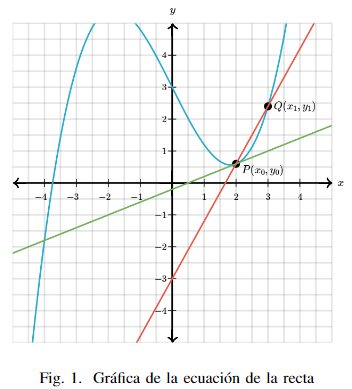
\includegraphics[width = 6 cm]{Latex-imágenes/GraficaEcuación.png}
    \caption{Gráfica de la ecuación de la recta}
    \label{fig:GraficaEcuacionRecta}
\end{figure}

Utilizando este método, es posible encontrar la ecuación de la recta a partir de dos puntos. Recordando que si los dos puntos son idénticos la recta será una linea vertical.

El algoritmo de solución para encontrar la ecuación de la recta pendiente  (ec. \ref{eqn:rectaPendiente}) comienza solicitando al usuario dos puntos $P(x_{1}, y_{1})$ y $Q(x_{2}, y_{2})$.\\

\centering
\begin{figure}[H]
    \centering
    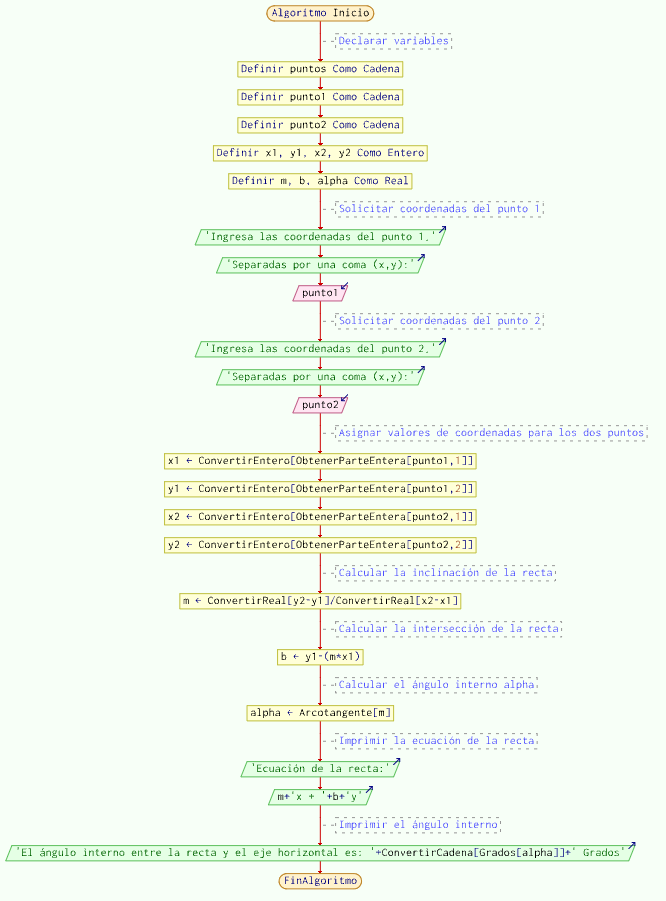
\includegraphics[width = 6 cm]{Latex-imágenes/Diagrama.png}
    \caption{Diagrama de flujo usado.}
\end{figure}


\subsection{\textbf{Desarrollo de la solución:}}
En el primer fragmento, se solicitan las coordenadas de dos puntos, A y B, que se ingresan en formato (x, y). Las coordenadas se leen como cadenas para separar las componentes x e y. Finalmente, se cierra el objeto Scanner para liberar los recursos.

\begin{javaCode}

Scanner puntos = new Scanner (System.in);
        
    //Solicitar puntos para la ecuacion de la recta  
    System.out.println("""
                        Ingresa las coordenadas del punto 1.
                        seperadas por una coma (x,y):
                           """);
    
    String[] punto1 =puntos.nextLine().split(",");
        
    System.out.println("""
                        Ingresa las coordenadas del punto 1.
                        seperadas por una coma (x,y):
                        """);
    
    String[] punto2 =puntos.nextLine().split(",");
        
    //cerrar el escaneo
    puntos.close();
        
\end{javaCode}

Las coordenadas separadas se convierten de cadenas a números enteros utilizando Integer.parseInt(). El método trim() se utiliza para eliminar cualquier espacio en blanco que pueda haber alrededor de las coordenadas.

\begin{javaCode}
    //Asignar valor de coordenadas a x,y para dos puntos
    int x1= Integer.parseInt(punto1[0].trim());
    int y1= Integer.parseInt(punto1[1].trim());
       
    int x2= Integer.parseInt(punto2[0].trim());
    int y2= Integer.parseInt(punto2[1].trim());
\end{javaCode}

Aquí se calcula la pendiente ($m$) de la recta utilizando la fórmula
\[
m = \frac{{y_2 - y_1}}{{x_2 - x_1}}
\]
y luego se calcula la intersección en el eje $Y$ ($b$) utilizando la fórmula.(ec. \ref{eqn:eqnRecta})
La ecuación de la recta resultante es\\ $y = mx + b$.

\begin{javaCode}
    //Calculo para la inclinacion de la recta  
    Double m = (double)(y2 - y1)/(x2 - x1);
       
    //Calcular Interseccion de la recta
    Double b= y1 -(m * x1);
\end{javaCode}
Se calcula el ángulo interno (\(\alpha\)) entre la recta y el eje horizontal utilizando la función \texttt{Math.atan(m)}. El resultado se convierte de radianes a grados.\\
\begin{javaCode}
    // Calcular el ángulo interno $\alpha$
        Double alpha = Math.atan(m);
        
\end{javaCode}
Finalmente, se imprime la ecuación de la recta y el ángulo interno en grados. La ecuación se imprime en formato \(mx + by\), y el ángulo se imprime en grados.
\begin{javaCode}
   //Imprimir ecuacion de la recta
        
        System.out.println("Ecuacion de la recta igual= \n" +
                 m + " x + " + b + " y ");
       //Imprimir el resultado de el ángulo interno 
        System.out.println("El ángulo interno entre la recta y el eje horizontal es: " 
                + String.format("%.3f", Math.toDegrees(alpha)) + " Grados");
                
\end{javaCode}
La función String.format() formatea un número decimal según el formato especificado en la cadena de formato.(En este caso 3f es el formato que indica que el número debe redondearse a tres). decimales
\subsection{\textbf{Depuración y pruebas:}}
\begin{table}[ht]
    \centering
    \begin{tabular}{|c|c|c|c|c|c|c|}
        \hline
        \textbf{Prueba} & \textbf{Punto 1} & \textbf{Punto 2} & \textbf{Pendiente (\(m\))} & \textbf{Intersección (\(b\))} & \textbf{Ángulo (\(\alpha\))} & \textbf{Ecuación de la Recta} \\
        \hline
        1 & (1, 2) & (3, 4) & 1.0 & 1.0 & 45.000 & \(y = x + 1\) \\
        \hline
        2 & (-1, 0) & (2, -3) & -1.0 & 1.0 & -45.000 & \(y = -x + 1\) \\
        \hline
        3 & (-4, 1) & (1, 4) & 0.6 & 3.4 & 30.964 & \(y = -x + 5\) \\
        \hline
        % Pruebas necesarias
    \end{tabular}
    \caption{Pruebas para el programa de ecuación de la recta}
    \label{tab:pruebas}
\end{table}